\chapter{News Feed System}

\ha{What is News Feed Systesm?}

A news feed is sytems that aggregate news/post/code other informatin from a set of post by other user/system. It thens shows them in desired order to the user. The system target is to provide information to the system user. One of the indirect goal of the system in to suggest content to user so that they will spend much of thier time on the web.

\hb{What the User can Post?}
User can post video,text,photo and other short info.


\hb{Real Life Use Case}
Some of the examples of system use are:
\ls
    \i Facebook News Feed System
    \i Instrgram Feed
    \i Google News Feed (data is generated from web itself)
    \i Twitter Timeline
\le

\ha{Design Scope Aggrement}
We will be asking question to decide how complex our system need to be. Also we will clarify any question regarding the system and performace and user expectatino.

\ha{Functional Features}
\lstart
    \i What the user is allowed to post?
    \r{user can post video,photo,text and external links}

    \i Can other user like,dislike ,post and comment on the post?
    \r{Yes, but its secondard to your explanation as main features will be post and timeline.}

    \i DAU? 
    \r{Lets suppose its 1B}

    \i Do we need storage?
    \r Yes, lets suppose we need storeage for 5 years.

    \i Are we designing mobile only app? web app? or both?
    \r Its both, giving user the flexibility to use the system at their convience.

\lend

\hb{Non Functional Features}
\lstart
    \i Its okay if uploading of a video takes a little time.
    \i Timeline generation should not take long,as it will user experience and user may leave the app.
    \i post of celebrity need to take special care.
    \i generation of timelint at runtime is expensigve, so we need to pre-compute it on our desing.
\lend

\ha{HLD Proposal}
Once we have basic understanding of the system, we can now propose initial desing. This way we can be sure that we and the interviewer agree on what is expected from the system.

There are two main featuers of our system (a) Post Services (b) Timeline Generation.

% TO-DO: Decrease pic resolution for fast compilation
    \b{HLD Diagram}\\
    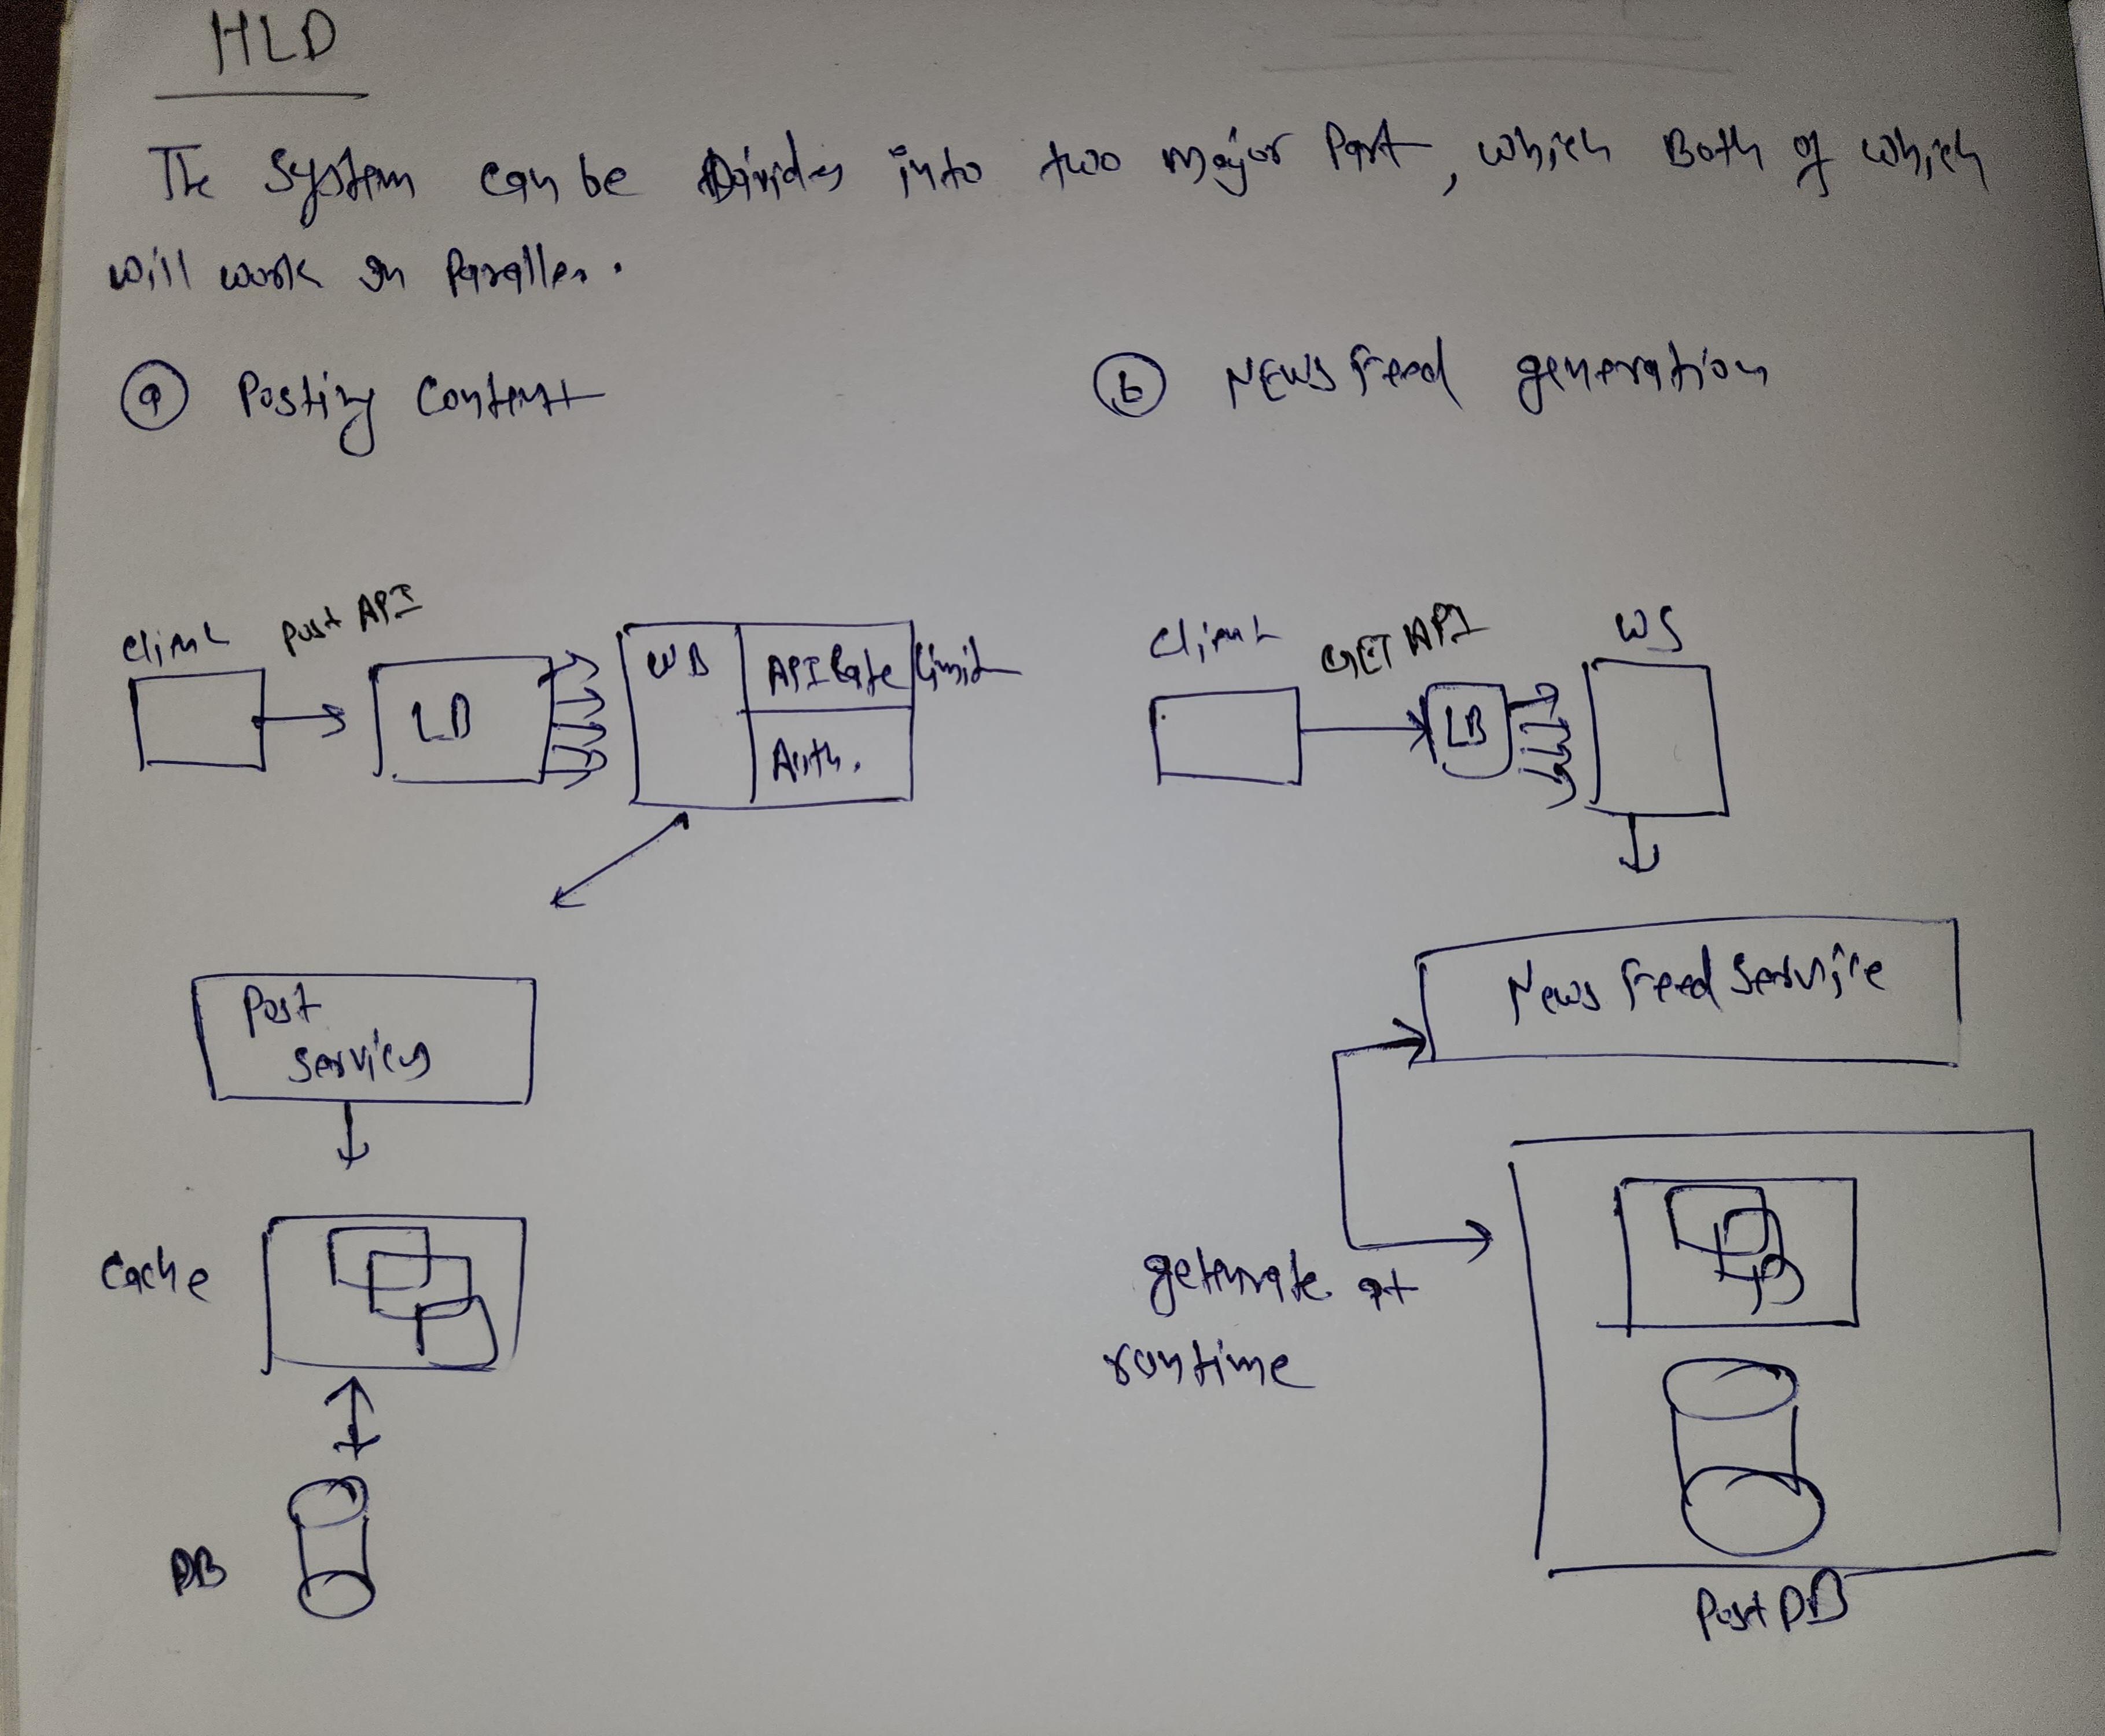
\includegraphics[width=0.7\textwidth]{resources/news-feed-hld.jpg}    



For posting, we will have our clients at either mobile/web. They will be post via exposed REST postAPI. They will be call the API and post the content. Once the webserver receives it forward the postrequest to postServices. It then save the data to DB, which is backed by cache.

For timeline generation, once the user opens the app then he will query the server. The server will check their friend list and their post,like etc and generate a JSON timeline response and send it to user.


\ha{HLD Evolution and LLD}
As we can observer there are various thing that make user experiance bad, and we can imporve them. Some of them are:
\lstart
    \i News Feed generation at run-time will take too much time. 
    \r We proposed alternative solution, in which news feed will be precomputed to save loading time on user time. Once any user post anything, then we pass that info to a new module called \u{Fanout Service}. The fanout service will get the user post and their friend list, and generate a (postID,userID) pair and push them into a queue. A set of worker thread keep reading this queue, it extracts a pair from the queue.And update userID timeline with consideration for the newly post. (if it want extra data it can query corresponding DB to get postDetails or userDetaisl.)

    \i With above approach, if the user has many friends / user the follow them. That that will lead to a heavy-increase in queue size, overall slowing the system. For these type of user, we will follow \u{Fanout on Read} instead of \u{Fanout On Write}. Once the user open their timeline, then recent post are pulled when user loads her homepage.

    \i For less-active user(who follows a celebrity), fanout on write works best. As computing resources are not waisted.

    \i How can we get list of friends?
    \r Instead of using SQL/No-SQl db, we use will be using \b{graphDB}  which works better with relationship data.

    \i Discuss userCache, postCache and newsFeedCache.
    \r These cases will be stored in front of DB, and instead of storing whole db-row, we will save metadata on the cache. (As original post is needed only if user loads the homepage, in all precomuption steps only their ID are sufficent.)

    \i Do we need CDN?
    \r Yes, as we know from socal media user want to see popular content. So if we place CDN also, static data load(like mangalyaan-3 landing) can be loaded fast.

    \i As we know we will need to be shard the userDB. Discuss the partiotioning strategy for best performace of the userDB and postDB.
\lend

\textbf{News Feed LLD}\\
\includegraphics[width=\textwidth]{resources/drawio/news-feed-lld.png}

\ha{Further Discussion Point}
As every system is complex, there will always be imporvement points. Some of the points can be applied to any system.
If time permits you can discuss and evolve the desing around these points alos:\

\hb{Scaling the DB}
\ls
    \i Vertical Scaling vs Horizontal Scaling
    \i SQL  vs No-SQL vs graphDB
    \i Master-Slave Replication and other replication strategy
    \i Read Replice and their use
    \i Consistely Models
    \i Databsse Sharding and avoiding common db problem like: hotspot problem
\le

\hb{Scaling the Desing}
\ls
    \i Keeping web tier stateless
    \i Caching and cache evicatioh policy and types of cache
    \i Use of multiple data center
    \i loose couple component with mesage queues
    \i Monitoring Features. (ex: QPS during peak hours, maximumm queue size etc)
    \i use of Notifcation system when post is generated.
\le
